%%%%%%%%%%%%%%%%%%%%%%%%
%%%%%   Präambel   %%%%%
%%%%%%%%%%%%%%%%%%%%%%%%

\documentclass[a4paper,
12pt,
oneside]
{article}

%%% Imports %%%

% Deutscher (und englischer) Zeichensatz
\usepackage[utf8]{inputenc}
\usepackage[english, ngerman]{babel} % Englisch als Sekundärsprache

% Schriftart Helvetica
\usepackage[scaled]{helvet}
\usepackage[T1]{fontenc}%Fonts in westeuropäischer Codierung (vor allem Sonderzeichen)

% Seitenränder
\usepackage[left=4cm,
right=2cm,
top=4cm,
bottom=2cm]
{geometry}

% Zeilenabstände
\usepackage{setspace}

% Kopf- & Fußzeile
%\usepackage{fancyhdr}
\usepackage[bottom]{footmisc} % Fußzeile immer am Boden 

% Schriftgröße & Abstände der Überschriften anpassen
\usepackage{sectsty}
\usepackage{titlesec}

% Grafiken
\usepackage{graphicx}
\usepackage{wrapfig}

% Abkürzungsverzeichnis
\usepackage{acronym}

% Links
\usepackage[hyphens]{url}
\usepackage{etoolbox}

% Farben
\usepackage{xcolor}

% Upquote
\usepackage{upquote}

% 
\usepackage{accsupp}

% Code-Block
\usepackage{listings}

% Dinge am Boden ausrichten
\usepackage{dblfloatfix}





%%% Meta-Daten %%%
\author{David Bährens}
\title{Portfolio Nr. 6 - Überprüfung und Verarbeitung eines String mit ASP.Net}



%%% Befehle neu definieren %%%
\renewcommand\familydefault{\sfdefault} % Helvetica einbinden
% \indivskip erzeugt einen 6pt großen Zeilenabstand nach einem Absatz %
\newcommand{\sPar}{\par\vspace*{6pt}}



%%% Formatierung %%%
\onehalfspacing

% Links
\urlstyle{same}
\appto\UrlBreaks{\do\a\do\b\do\c\do\d\do\e\do\f\do\g\do\h\do\i\do\j
	\do\k\do\l\do\m\do\n\do\o\do\p\do\q\do\r\do\s\do\t\do\u\do\v\do\w
	\do\x\do\y\do\z}

% Codeblock - Zeilennummern nicht kopierbar
\newcommand{\noncopynumber}[1]{%
	\BeginAccSupp{method=escape,ActualText={}}%
	#1%
	\EndAccSupp{}%
}



%%% Kopf- & Fußzeile %%%
\pagestyle{myheadings}



%%% Literaturverzeichnis %%%
\makeatletter
\renewcommand\@biblabel[1]{}
\makeatother



%%% Farben %%%
\definecolor{editorGray}{rgb}{0.95, 0.95, 0.95}
\definecolor{editorOcher}{rgb}{1, 0.5, 0} % #FF7F00 -> rgb(239, 169, 0)
\definecolor{editorGreen}{rgb}{0, 0.5, 0} % #007C00 -> rgb(0, 124, 0)
\definecolor{mint}{rgb}{0.24, 0.71, 0.54}
\definecolor{gray}{rgb}{0.5, 0.5, 0.5}



%%% Programmiersprachen %%%
\lstdefinelanguage{HTML5}{
	language=html,
	sensitive=true, 
	alsoletter={<>=-/:@{}},
	keywords={ true, false, {{, }}, <h1>, </h1>, <form, <br>, <input, </form>, <p>, </p>, <h2>, </h2>, <p, <title>, </title>, <meta, >, <html, <head>, </head>, <body>, </body>, </html>, <span, </span>, <span> }
	ndkeywords={
		% General
		=,
		% HTML attributes
		charset=, id=, width=, height=, src=, name=, content=, action=, method=, type=, style=, lang=, asp-for=, 
		% CSS properties
		border:, transform:, -moz-transform:, transition-duration:, transition-property:, transition-timing-function:,
		%Vue.js
		v-model=, @keyup=, @keydown=, v-on:click=, v-if=
	},
	morecomment=[s]{<!--}{-->},
	tag=[s]
}

\lstdefinestyle{cshtml} {
	% Basic design
	backgroundcolor=\color{editorGray},
	basicstyle={\footnotesize\ttfamily},
	columns=fullflexible,   
	frame=single,
	rulecolor=\color{black},
	% Line numbers
	numbers=left,
	stepnumber=1,
	firstnumber=1,
	numberfirstline=true,
	numberstyle=\tiny\color{gray}\noncopynumber,
	% Code design   
	commentstyle=\color{mint}\ttfamily\textit,
	ndkeywordstyle=\color{red}\bfseries,
	keywordstyle=\color{blue}\bfseries,
	stringstyle=\color{editorOcher},
	% Code
	language=HTML5,
	%alsolanguage=JavaScript,
	tabsize=4,
	%alsodigit={.:;},
	showspaces=false,
	showstringspaces=false,
	extendedchars=true,
	breaklines=true,        
	% Support for German umlauts
	literate=%
	{Ö}{{\"O}}1
	{Ä}{{\"A}}1
	{Ü}{{\"U}}1
	{ß}{{\ss}}1
	{ü}{{\"u}}1
	{ä}{{\"a}}1
	{ö}{{\"o}}1
}

\lstdefinestyle{csharp} {
	% Basic design
	backgroundcolor=\color{editorGray},
	basicstyle={\footnotesize\ttfamily},
	columns=fullflexible,   
	frame=single,
	rulecolor=\color{black},
	% Line numbers
	numbers=left,
	stepnumber=1,
	firstnumber=1,
	numberfirstline=true,
	numberstyle=\tiny\color{gray}\noncopynumber,
	% Code design   
	commentstyle=\color{mint}\ttfamily\textit,
	ndkeywordstyle=\color{red}\bfseries,
	keywordstyle=\color{blue}\bfseries,
	stringstyle=\color{editorOcher},
	% Code
	language=[Sharp]C, 
	%alsolanguage=JavaScript,
	tabsize=4,
	%alsodigit={.:;},
	showspaces=false,
	showstringspaces=false,
	extendedchars=true,
	breaklines=true,        
	% Support for German umlauts
	literate=%
	{Ö}{{\"O}}1
	{Ä}{{\"A}}1
	{Ü}{{\"U}}1
	{ß}{{\ss}}1
	{ü}{{\"u}}1
	{ä}{{\"a}}1
	{ö}{{\"o}}1
}


\DeclareRobustCommand\squelch[1]{%
	\BeginAccSupp{method=plain,ActualText={}}#1\EndAccSupp{}}





%%%%%%%%%%%%%%%%%%%%%%%%%
%%%%%   Main Part   %%%%%
%%%%%%%%%%%%%%%%%%%%%%%%%

\begin{document}
	\pagenumbering{Roman}
	\begin{titlepage}
		\begin{center}
			\textbf{\huge Portfolio Nr. 6 - Überprüfung und Verarbeitung eines String mit ASP.Net} \\ \vspace{1.5cm}
			{\LARGE Portfolio} \\ \vspace{1cm}
			{\large
				Fakultät für Wirtschaft \\
				Studiengang Wirtschaftsinformatik \\
				Studienjahrgang 2018 \\ 
				Kurs C} \\ \vspace{1cm}
			\textsc{\LARGE 
				Duale Hochschule Baden-Württemberg \\
				Villingen-Schwenningen} \\ \vspace{1.5cm}
			\large
			\begin{minipage}[t]{.48\textwidth}
				Bearbeiter: \\
				David Bährens \\
				\\
				Dualer Partner: \\
				DATEV eG \\
			\end{minipage}
			\begin{minipage}[t]{.48\textwidth}
				Betreuender Dozent: \\
				Prof. Dr. Kimmig \\
			\end{minipage}
			\\ \vspace{0.5cm}
			\begin{minipage}[t]{.48\textwidth}
				
\includegraphics[width=4cm]{img/datev.png}
			\end{minipage}
			\begin{minipage}[t]{.48\textwidth}
				
\includegraphics[width=8cm]{img/dhbw.png}
			\end{minipage}
		\end{center}
	\end{titlepage}
	\clearpage
	
	
	
	\thispagestyle{empty}
	\setcounter{page}{2}
	\tableofcontents
	\clearpage
	
	
	
	\section*{Abkürzungsverzeichnis}
	\addcontentsline{toc}{section}{Abkürzungsverzeichnis}
	\begin{singlespace}
		\begin{acronym}[asdfasdfasdf]
			\acro{Abb.}{Abbildung}
			\acro{ASP}{Active Server Pages}
			\acro{FCL}{Framework Class Library}
			\acro{CLR}{Common Language Runtime}
			\acro{UI}{User Interface}
			\acro{OS}{Operating System}
			\acro{MS}{Microsoft}
			\acro{z. B.}{zum Beispiel}
			\acro{API}{Application-Programming-Interface}
			\acro{ASP}{Active Server Pages}
			\acro{REST}{Representational State Transfer}
			\acro{MVC}{Model-View-Controller}
			\acro{VS}{Visual Studio}
			\acro{SPA}{Single Page Application}
			\acro{Z.}{Zeile}
			\acro{RP}{Razor Page}
		\end{acronym}
	\end{singlespace}
	\clearpage
	
	
	
	\addcontentsline{toc}{section}{\listfigurename}
	\listoffigures
	\clearpage
	
	
	
	\pagenumbering{arabic}
	
	\section{Einleitung}
	\clearpage
	
	
	
	
	\section{Theoretische Grundlagen}
	
	\subsection{ASP.Net}
	Bei ASP.Net handelt es sich um ein modulares und serverseitiges Web-Framework zur Entwicklung von dynamischen Web-Anwendungen. ASP steht für \glqq Acrive Server Pages\grqq. Dieses ist Teil des Microsoft (MS) Softwareentwicklungs und Execution-Framework .Net. .Net dient unter Windows zur Erstellung von Anwendungsprogrammen. Dessen wesentlichen beiden Bestandteile sind zum einen die Framework Class Library (FCL) und die Common Language Runtime (CLR). FCL ist eine umfangreiche Klassenbibliothek in .Net. Sie enthält beispielsweise User Interface (UI)-, File Access- oder Netzwerk-Kommunikationsklassen. Bei CLR handelt es sich um die Laufzeitumgebung in der .Net Anwendungen ausgeführt werden. .Net Programme, beispielsweise eine C\# Anwendung, greifen nicht direkt auf das Betriebssystem (OS) zu. Stattdessen wir der Programmcode in die sogenannte  MS Intermediate Language Assemby kompiliert und dann in der CLR ausgeführt. Die CLR wiederum greift dann direkt auf das darunterliegende OS zu (siehe Abb. \ref{fig:dotnet}).\footnote{Vgl. Beasley, Robert E., .Net Basics, 2020, S. 8}
	\begin{figure}[h]
		\centering
		\caption{.Net Framework}
		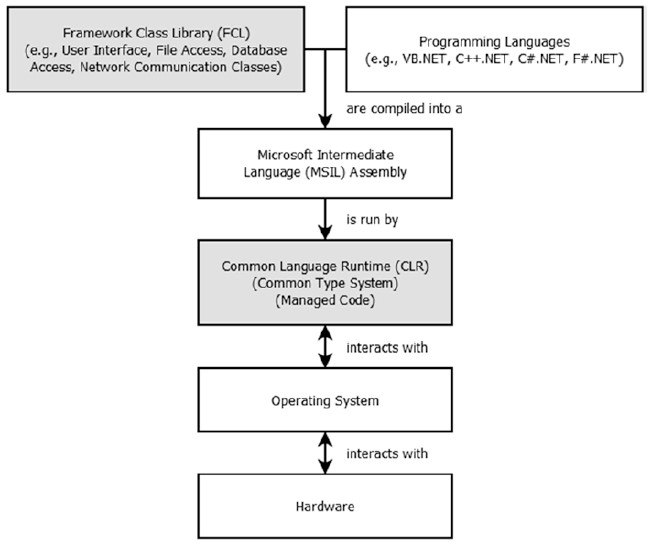
\includegraphics[width=11.5cm]{img/dotnet.jpg} \\
		\vspace{5pt}
		\footnotesize{Quelle: Beasley, Robert E., .Net Basics, 2020, S. 9}
		\label{fig:dotnet}
	\end{figure} \\
	Das .Net Framework wird jedoch fortlaufend durch .Net Core abgelöst. Hierbei handelt es sich um eine Open-Source-Plattform von MS und eine Modernisierung des .Net Frameworks. Ein besonderer Vorteil dieses moderneren Frameworks ist seine Plattformunabhängigkeit. Da ASP.Net auf .Net basiert erfolgt die Ablösung hier analog mit ASP.Net Core.\footnote{Augsten, Stephan, .Net Core, 2020} \sPar
	ASP.Net wiederum stellt verschiedene Frameworks für die Entwicklung von Web-Anwendungen zur Verfügung. Die wichtigsten sind Folgende. Zum einen gibt es das inzwischen veraltete, ereignisgesteuerte Framework \glqq Web Forms\grqq. Bei diesem wurden Oberflächen über einen Designer mit einer Drag-and-Drop Mechanik erstellt und die Logik wurde über einen Eventhandler implementiert. In der Vergangenheit kam Web Forms jedoch teilweise mit der Zustandslosigkeit des Webs in Konflikt. \\
	Ein moderneres, aktionsgesteuertes Framework stellt dagegen ASP.Net MVC dar. Dieses folgt den MVC Pattern, wodurch UI, Logik und Daten voneinander getrennt werden. MVC steht dabei für die drei wesentlichen Bestandteile in die eine MVC-Anwendung zerlegt wird, \glqq Model-View-Controller\grqq. Das Model gibt dabei die Datenstruktur, die View die Darstellung bzw. die UI und der Controller beinhaltet die Logik und verbindet das Model mit der View.\footnote{Rouse, Margaret, MVC, 2016} \\
	Dann sind da noch die Web Pages, die über die neue Razor Syntax verfügen. Razor Pages (RP's) sind eine moderne Alternative zur Entwicklung von dynamischen Websites und sie stellen den Nachfolger von ASP.Net MVC dar. Sie werden in einem gesonderten Kapitel erläutert, da sie für diese Arbeit von größerer Bedeutung sind. \\
	Zuletzt ist noch ASP.Net Web API zu nennen, mit dessen Hilfe Web-Schnittstellen wie z. B. REST entwickelt werden können.\footnote{Gutsch, Jürgen, ASP.Net, 2017} \sPar
	Die .Net Entwicklung ist mit einer Reihe kompatibler Programmiersprachen möglich. Hierzu zählen beispielsweise Visual Basic, C\# oder F\#. Diese Arbeit bezieht sich im folgenden lediglich auf C\#. C\# ist eine objektorientierte und typsichere höhere Programmiersprache von MS. Ursprünglich war sie primär auf Windows ausgerichtet, inzwischen ist sie jedoch sehr universell und kann für die Entwicklung von Web-Apps eingesetzt werden.\footnote{Augsten, Stephan, C\#, 2019}
	
	
	
	\subsection{Razor Pages}
	
	RP's basieren auf ASP.Net MVC und zeichnen sich durch die Razor Syntax aus. Mit dieser können statische HTML Webseiten mit C\# dynamisch gemacht werden. Dies zeichnet sich dadurch aus, dass eine Webseite durch eine .cshtml Datei erstellt wird, also eine Kombination aus C\#, mittels der Razor Syntax und HTML. Der dort enthaltene Code wird dabei serverseitig in reines HTML übersetzt. RP's vereinen die Vorteile einer verhältnismäßig einfachen Syntax mit einem leichtgewichtigen und dennoch mächtigen Framework. Anders als ASP.Net MVC nutzen RP's das Model-View-ViewModel-Pattern statt echtem MVC. Hierbei handelt es sich um eine spezielle Form der MVC-Architektur, bei der kein Controller, sondern stattdessen ein ViewModel, das bei RP's PageModel genannt wird, eingesetzt wird. Dieses ist eine spezielle Implementierung eines Controllers, welcher die Logik und Programmcode hinter einer View darstellt. Jede View hat ein eigenes ViewModel, statt einem zentralen Controller, der alle Views steuert. Model und View funktionieren analog zu ihrer Funktionalität bei MVC. Die View erhält ihre benötigten Daten dabei mittels Data Binding. Analog zu MVC ist der Zweck MVVM's die Trennung von Logik, UI und Daten. Diese erfolgt bei MVVM allerdings seitenbasiert.\footnote{o. V., MVVM, 2017} RP's sind automatisch auch bei einem ASP.Net MVC Projekt aktiviert und anders herum kann auch in einer RP mit der MVC-Architektur gearbeitet werden falls dies gewünscht wird. \footnote{o. V., RP's, 2019}
	
	\subsubsection{Aufbau eines Razor Page Projektes}
	Ein Standard Razor Projekt besteht aus verschiedenen unterschiedlichen Dateien (siehe Abb. \ref{fig:aufbau}). Die wohl wichtigsten befinden sich in dem \glqq Page\grqq~Ordner. Dieser enthält .cshtml Dateien und .cshtml.cs Dateien. Die .cshtml Dateien sind die Views bzw. die eigentliche RP. Mit Hilfe der Razor Syntax könnte hierin auch Logik implementiert werden und somit jeglicher Quellcode in einer Datei gebündelt werden. Dies widerspricht allerdings dem Prinzip der Datentrennung bei MVVM und ist kein guter Programmierstil. Die .cshtml.cs dagegen sind die PageModels der RP. Diese können sowohl die Datenstruktur, als auch die Logik beinhalten. Dies erkennt man im Übrigen auch aus der Abbildung \ref{fig:aufbau}, da hier offensichtlich kein separates Model implementiert wurde. Ein solches würde, falls benötigt, in einem separatem Model-Ordner, direkt unter dem Wurzelverzeichnis implementiert werden. Diese sind, genau wie die PageModels, C\# Dateien. PageModels vereinen damit eine breite Menge an Funktionalitäten, wie beispielsweise HTTPContext, den ModelState oder die Behandlung von Requests und Responses, wie z. b. HTTP-Anfragen, die in MVC getrennt würden.\footnote{Jones, Matthew, Razor vs. MVC, 2019} Der Startpunkt der Website bildet die Index.cshtml. Eine weitere wichtige Page-Datei ist die \_Layout.cshtml, welche ein Design-Template für jede andere Page darstellt. In ihr kann z. B. der Header der Website für alle RP's festgelegt werden. Insgesamt erfüllen Pages mit einem \glqq\_\grqq~als Präfix jeweils eine besondere Aufgabe, sind allerdings nicht über einen URL-Aufruf erreichbar. Der Aufruf von \glqq https://Hostname/\_Layout\grqq~z. B. würde daher zu einem 404 Http Error führen.
	\begin{wrapfigure}{r}{7cm}
		\centering
		\caption{Aufbau Razor Pages} 
		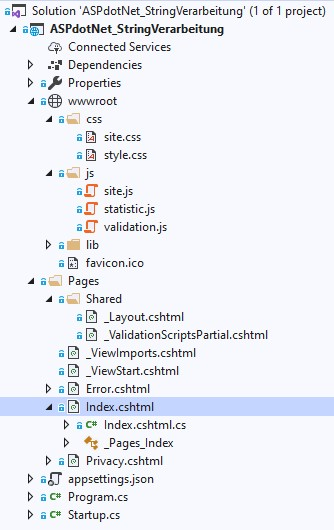
\includegraphics[width=7cm]{img/aufbau.jpg} \\
		\label{fig:aufbau}
	\end{wrapfigure}
	Offensichtlich werden RP's, anders als bei ASP.Net MVC, Dateien nach dem Zweck gegliedert. Es gibt nicht nur einen Controller der die gesamte Geschäftslogik in sich vereint, sondern stattdessen gibt es viele C\# Dateien, PageModel darstellen und jeweils einer View zugeordnet sind. \\
	In wwwroot befinden sich statische Dateien, wie CSS-Style-Sheets, Bilder oder JavaScript(JS)-Dateien. Im lib Ordner wiederum befinden sich Drittanbieter-Pakete. Defaultmäßig sind dies JQuery und Bootstrap, was im Verlauf der Arbeit noch erläutert wird. \\
	Darüber hinaus befinden sich direkt in dem Wurzelverzeichnis eine Konfigurationsdatei im JSON-Format für die gesamte Anwendung namens \glqq appsettings.json\grqq, eine \glqq Program.cs\grqq, die den Startpunkt der Anwendung darstellt und nach eine \glqq Startup.cs\grqq. In letzterer können z. B. benötigte Services hinzugefügt und weitere Konfigurationen vorgenommen werden.\footnote{o. V., Aufbau RP's, 2020} Folgendes Beispiel zeigt, wie der RP Service in eine ASP.Net Webanwendung integriert werden können:
	\lstset{style=csharp}
	\begin{lstlisting}
 public void ConfigureServices(IServiceCollection services)
{
	services.AddRazorPages();
}
	\end{lstlisting}
	
	\subsubsection{Aufbau einer Razor Page}
	Eine RP zeichnet sich, wie bereits erwähnt, vor allem auch durch die Razor Syntax aus, die in den HTML-Code eingefügt wird. Der Server erkennt sie durch ein vorangestelltes \glqq @\grqq. So kann beispielsweise ganzer C\#-Code einfach in den HTML-Code eingefügt werden und ihn dadurch mit Funktinalität ausstatten. Dies geschieht innerhalb eines Codeblocks: \texttt{@\{ C\#-Code \}}. Darüber hinaus können auch einzelne Funktionen, wie eine if-Funktion, oder auch eine Schleife mit einem vorangestellten @ benutzt werden: \texttt{@if ( Condition ) \{ C\#-Code \}}. Es ist auch möglich von der View aus auf bestimmte Variablen des PageModels zuzugreifen. Dies geschieht über \texttt{@Model.variable}. Um auf diese Variable zugreifen zu können muss sie allerfings als Public deklariert werden. Eine weitere Möglichkeit, Daten vom PageModel an die View zurückzugeben ist ViewData, wobei es sich um ein dictionary verschiedener Objekte handelt. Dieses dictionary wird automatisch an die View übergeben. Somit kann jederzeit auf die darin enthaltenen Objekte, über den jeweiligen Key, zugegriffen werden. ViewData Attribute werden wie folgt im Page Model definiert und anschließend über \texttt{@ViewData["Key"]} aufgerufen.\footnote{o. V., ViewData, o. D.}
	\lstset{style=csharp}
	\begin{lstlisting}
public class IndexModel : PageModel
{
	[ViewData]
	public string Key { get; set; }
	// Oder alternativ
	ViewData["Key"] = "Value"
}
	\end{lstlisting}
	Außerdem existieren verschiedene Tag-Helpers, also wiederverwendbarer HTML-Code für die Vereinfachung von ASP Funktionalitäten. Ein Beispiel hierfür wäre der Validation Message Tag Helper \texttt{asp-validation-for}, der einem span-Element eine Validation Error Message zuordnet, indem er ihm das HTML-Element \texttt{data-valmsg-for} zuweist. Bei einem Client seitigen Validationsfehler zeigt jQuery die Fehlermeldung innerhalb des spans. Der Tag kann allerdings auch für eine serverseitige Validation verwendet werden. Diese könnte beispielsweise so aussehen: 
	\lstset{style=cshtml}
	\begin{lstlisting}
<input type="text" asp-for="IBAN" />
<span asp-validation-for="IBAN"> </span>
	\end{lstlisting}
	\lstset{style=csharp}
	\begin{lstlisting}
public class IndexModel : PageModel
{
	[BindProperty]
	[Required]
	public string IBAN { get; set; }
}
	\end{lstlisting}
	Wurde nun keine IBAN, bei einem Request an den Server, eingegeben wird unterhalb des Textfeldes eine Fehlermeldung ausgegeben. Ein weiteres Beispiel wäre der \texttt{asp-page-handler}, mit dem ein spezieller Page Handler ausgeführt werden kann. Bei Handler Methoden handelt es sich um Funktionen, die automatisch bei einem entsprechenden HTTP-Request ausgeführt werden. Die Handler Methode \texttt{OnGet()}~wird beispielsweise bei einer Get-Anfrage an den Server ausgeführt. Mit dem \texttt{asp-page-handler} können nun verschiedene Page Handler implementiert werden. So würde ein  \texttt{OnPostProcessing()}~Handler nur bei einem bestätigen von \texttt{<button type=\glqq submit\grqq~asp-page-handler=\glqq Processing\grqq>Submit</button>} ausgeführt werden.\footnote{o. V., Page Handler, 2018} \footnote{Anderson, Rick; Mullen, Taylor; Vicarel, Dan, Razor Syntax, 2020} \\
	Jede Page beginnt stehts mit \texttt{@page} in der ersten Zeile. Hierdurch weiß ASP.Net, dass es diese datei wie eine RP behandeln muss. Hierdurch kann die Page selber Aktionen ausführen und ist nicht auf einen Controller angewiesen. Des Weiteren muss ein \texttt{@model} angegeben werden, mit dem dazugehörigen Model dieser View. Bei RP's ist dies in der Regel (i. d. R.) das PageModel.\footnote{Jones, Matthew, Razor vs. MVC, 2019}
	
	
	
	\subsection{Bootstrap}
	 \begin{wrapfigure}{r}{5.5cm}
	 	\centering
	 	\caption{Bootstrap in Razor Page Projekt mit VS} 
	 	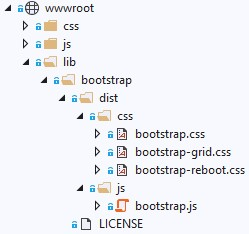
\includegraphics[width=5.5cm]{img/bootstrap_asp.jpg} \\
	 	\label{fig:bootstrap_asp}
	 \end{wrapfigure}
	Bei Bootstrap handelt es sich um ein Frontend-Framework zur optischen Gestaltung einer Website. Es dient primär der schnellen und einfachen Umsetzung eines Responsive Web-Designs, mit dem Websites für jede Displaygröße optimal gestaltet sein sollen. Damit verfolgt Bootstrap stark die Mobile-first Philosophie. Ursprünglich handelte es sich bei Bootstrap um eine Technologie von Twitter, die dann als Open-Source-Projekt veröffentlicht wurde. Wenn man sich seine Bestandteile anschaut, dann basiert es überwiegend auf CSS, aber auch auf HTML und JS. Seine Bestandteile sind zum einen das Design von Basis-HTML-Elementen und JS Plugins, welche zumeist auf jQuery basieren, bei dem es sich um eine freie JS-Bibliothek handelt. 
	Darüber hinaus gibt es noch verschiedene Komponenten, bei denen es sich um von Bootstrap vordefinierte CSS-Klassen zur Gestaltung von HTML-Elementen handelt. Bootstrap ist zudem leicht anpassbar, sollten die vordefinierten Gestaltungsmöglichkeiten nicht den eigenen Wünschen entsprechen, wie wenn man beispielsweise ein neues Farblayout implementieren möchte.\footnote{Bhaumik, Snig, Bootstrap, 2015, S. 7-11} \sPar
	Bootstrap eignet sich besonders gut für die ASP.Net Einbindung, denn bei der Erstellung eines Standard RP Projektes mit Visual Studio (VS) ist Bootstrap bereits vorinstalliert und kann direkt verwendet werden (siehe Abb. \ref{fig:bootstrap_asp}).
	\clearpage
	
	
	
	
	
	\section{Praxisteil: Dokumentation und erklärung des Codes}
	
	\subsection{Grundfunktionalität}
	Die Grundfunktinalität beinhaltet eine ASP.Net-Webanwendung, in der der Benutzer eine beliebige Zeichenkette, die mindestens aus zehn Wörtern bestehen muss, eingeben kann. In dieser Zeichenkette sollen dann alle Vokale durch \glqq i\grqq~ersetzt werden. Die Eingabe muss validiert werden, sodass der Nutzer nicht weniger als zehn wörter eingibt. Diese Anwendung wurde als Single Page Application (SPA) realisiert. Das verwendete Framework für diese Aufgabe waren RP's. Diese Wahl liegt vor allem in der Einfachheit des Frameworks begründet. Da es sehr \glqq seitenbasiert\grqq ist und wegen der Razor Syntax ist es relativ einfach hiermit eine SPA umzusetzen. Das ASP.Net MVC Framework wäre hierfür unnötig kompliziert und die erhöhte Datentrennung wäre für ein solches Projekt nicht sinnvoll. \\
	Da es sich um eine SPA handelt, wurde, aus Vereinfachungsgründen, lediglich die Index-Datei als RP verwendet und keine zusätzlichen erstellt. \sPar
	Zunächst musste die Website für eine SPA vorbereitet werden. Die einfachste Möglichkeit dies umzusetzen ist, indem sich der RP Syntax bedient wird. Hierzu wurde ein boolean namens \glqq started \grqq, der defaultmäßig false ist, im PageModel angelegt und eine if-Bedingung hierzu in der View erstellt. Wenn diese Variable false ist, wird ein Startbildschirm mit einem Startbutton angezeigt. Bei einem Klick auf diesen wird die Variable auf true gesetzt, die if-Bedingung damit wahr und die eigentliche Anwendung wird angezeigt. Dies geschieht über den bereits erwähnten \texttt{aps-page-handler}. Dieser Tag helper, wurde dem Startbutton hinzugefügt. Auf Klick ruft er die Handler Methode \glqq OnPotStarting()\grqq~auf, in der die Variable started auf true gesetzt wird und danach die Website erneut zurückgegeben wird. Beim zurückgeben der Page wird die Seite neu geladen, und da der Wert in der if-Bedinung nun true ist, wird die eigentliche Anwendung statt der Startseite angezeigt. Um sie wieder zu beenden ist auf der Anwendungsseite ein exit Buttton der die Variable wieder auf false setzt. Dieser funktioniert analog zum Startbutton
	\lstset{style=csharp}
	\begin{lstlisting}
// Wurde die Anwendung über den Startbutton gestartet, wird die eigentliche Anwendung angezeigt
@if (@Model.started)
{
	// Deaktiviert die Anwenung über den Handler OnPostExitPage()
	<button type="submit" asp-page-handler="ExitPage">Exit</button>
}
// Defaultmäßig wird erst mal die folgende Startseite angezeigt
else
{
<form method="post">
	<button type="submit" id="startButton" asp-page-handler="Starting">Anwendung starten</button>
</form>
}
	\end{lstlisting}
	\lstset{style=csharp}
	\begin{lstlisting}
public class IndexModel : PageModel
{
	// Variable, ob die Anwendung gestartet wurde oder nicht
	public bool started = false;
}

public IActionResult OnPostStarting()
{
	// aktiviert die Anwendung, indem die Startvariable true gesetzt wird und die RP returned wird
	started = true;
	return Page();
}
	\end{lstlisting} ~\sPar
	Hiernach wird die Grundfunktionalität umgesetzt, welche in die if-Anweisung ab Zeile (Z.) vier des vorherigen Codes implementiert wird. Der Input erfolgt über eine textarea, die mittels DataBinding an das PageModel übergeben wird. Dort wird die Zeichenkette dann verarbeitet. Es existieren zwei Formen der Validierung. Eine clientseitige und eine serverseitige. Die clientseitige wurde mit HTML und Bootstrap realisiert. Sie validiert, ob überhaupt eine Eingabe erfoglt oder nicht. Hierzu wurden verschiedene Bootstrap-Klassen implementiert und das Attribut \texttt{required} zu der textarea hinzugefügt (Zeile 6). Bei einer fehlgeschlagenen Validierung wird Z. vier bis sechs ausgegeben. Damit diese Validierung funktioniert muss allerdigns noch JS hinzugefügt werden (siehe Anhang 1).
	\lstset{style=csharp}
	\begin{lstlisting}
<form method="post" class="needs-validation" id="inputForm" novalidate>
	<div class="input-group">
			<textarea asp-for="inputString" placeholder="Zeichenkette eingeben" class="form-control shadow-lg" aria-label="inputString" id="inputString" required></textarea>
		<div class="invalid-feedback">
			Bitte geben Sie eine Zeichenkette ein. Sonst funktionert das Ganze nicht...
		</div>
	</div>
	<button type="submit" asp-page-handler="Processing" form="inputForm">Absenden</button>
</form>
	\end{lstlisting} ~\\
	Bei der serverseitigen Validierung mit C\# mitteln wird überprüft, ob mindestens zehn wörter eingegeben wurden. Dies wird mit Regular Expressions (RegEx) überprüft. 
	\lstset{style=csharp}
	\begin{lstlisting}
[BindProperty]
[RegularExpression(@"(.*\s){9}..*", ErrorMessage = "Upps. Sie haben zu wenig Wörter eingegeben.")]
public string inputString { get; set; }
	\end{lstlisting} ~\\
	Stimmt die eingegebene Zeichenkette nicht mit der RegEx überein wird eine Fehlermeldung ausgegeben. Diese sollte allerdings abschreckender wirken, als die einfache \glqq required\grqq~Validierung. Daher wird sie an einer anderen Stelle ausgegeben und später mit Bootstrap gestaltet.
	Die Kennzeichnung, wo die Fehlermeldung stehen soll erfolgt mit \texttt{<span asp-validation-for=\glqq inputString\grqq></span>}. \\
	Nun muss der Input verarbeitet werden und alle Vokale durch ein \glqq i\grqq~ersetzt werden. Dies geschieht in der \glqq OnPostProcessing() \grqq~Handler-Methode. Da er nur verarbeitet werden soll, wenn die Validierung positiv war, wird diese in Z. 12 abgefragt. War sie positiv wird über jeden Buchstaben in der Zeichenkette iteriert und mit den Vokalen in dem \glqq vokale-Array\grqq verglichen. Ist ein Buchstabe in dem Vokale Array enthalten, wird er durch ein \glqq i\grqq~ersetzt (Z. 14-24). Der dadurch neu entstandene String wird in Zeile 28 zurückgegeben. Außerdem wird beim eingeben des Wortes \glqq exit\grqq der User auf die Startseite zurück geleitet (Z. 5-10).
	\lstset{style=csharp}
	\begin{lstlisting}
char[] vokale = { 'a', 'e', 'o', 'u' };
string[] words = { };

public IActionResult OnPostProcessing()
{
	inputString = inputString.ToLower();
	words = inputString.Split(" ");
	
	if (words.Contains("exit"))
	{
		return RedirectToPage("/index");
	}
	
	if (ModelState.IsValid)
	{
		foreach (var character in inputString)
		{
			if (vokale.Contains(character))
			{
				newChar = 'i';
				newString += newChar;
			}
			else
			{
				newString += character;
			}
		}
	}
	
	ViewData["result"] = newString;
	return Page();
}
	\end{lstlisting} ~\\
	Das Ergebnis wird nun in der View angezeigt. Dabei soll überprüft werden, ob die Validierung positiv oder negativ war. War sie positiv wird, der neue String angezeigt, ansonsten die bereits erwähnte Validierungsfehlermeldung. Es musste hierzu eine weitere Variable \glqq activated\grqq eingeführt werden, die defaultmäßig false ist und beim ersten ausführen von OnPostProcessing() true gesetzt wird. Dies liegt daran, dass ansonsten zu Beginn er Anwendung die textarea bereits validiert würde und eine Fehlermeldung ausgegeben wurde, obwohl der Benutzer noch gar nicht die Möglichkeit hatte eine Eingabe zu tätigen.
	\lstset{style=cshtml}
	\begin{lstlisting}
@if (@ModelState.IsValid)
{
	<code>@ViewData["result"]</code>
}
else if (!@ModelState.IsValid && @Model.activated)
{
	<span asp-validation-for="inputString"></span>
}
	\end{lstlisting} ~\\
	
	
	
	
	\subsection{Erweiterungen}
	Die primäre Erweiterung stellt eine Historie dar, in der alle eingegeben Zeichenketten, mit der veränderten neuen Zeichenkette ausgegeben werden und die bei Beenden der Anwendung gelöscht wird. Darüber hinaus gibt es eine kleine Statistik, die u. a. mit Google Charts visualiesiert wurde, der man entnehmen kann welche Vokale wie häufig mit dem Buchstaben \glqq i\grqq ersetzt wurden.
	
	\subsubsection{Historie}
	Um die Historie umzusetzen muss eine statische Variable angelegt wird, die auch nach einer POST-Anfrage nicht gelöscht wird (Z. 2) Der \texttt{historyEntry}-Liste wird dann einfach am Ende jedes Aufrufes der OnPostProcessing() Handler-Methode die Variable \texttt{inputString}, also die eingegebene Zeichenkette und die Variable \texttt{newString}, also die überarbeitete Zeichenkette hinzugefügt und diese wiederum der zweidimensionalen Liste \texttt{history} hinzugefügt. Danach wird \texttt{historyOutput = history} gesetzt, da so einfacher in der View auf die Variable zugegriffen werden kann.
	\lstset{style=csharp}
	\begin{lstlisting}
List<string> historyEntry = new List<string>();
static List<List<string>> history = new List<List<string>>();
public List<List<string>> historyOutput = new List<List<string>>();
	\end{lstlisting} ~\\
	In der View wird dann mit einer foreach-Schleife über die Liste iteriert und eine Tabelle mit den einzelnen Werten erstellt.
	 \lstset{style=cshtml}
	 \begin{lstlisting}
@if (@Model.activated)
{
	<table>
	<!-- ... -->
	@foreach (var entry in @Model.historyOutput)
	{
		<tbody>
			<tr>
				<td>@entry[0]</td>
				<td>@entry[1]</td>
			</tr>
		</tbody>
	}
	</table>
}
	 \end{lstlisting} ~\\
	 Zuletzt muss die Historie bei jedem Beenden der Anwendung ebenfalls gelöscht werden. Dies geschieht zum Einen in der bereits erwähnten Handler-Methode OnPostExitPage(), indem die statische Variable \texttt{history} einfach mit \texttt{history = new List<List<string>>();} neu initialisiert wird. Zum anderen muss diese Initialisierung auch in die bereits erwähnte if-Bedingung, zur Überprüfung, ob das Wort \glqq exit\grqq~eingegeben wurde, hinzugefügt werden:
	 \lstset{style=csharp}
	 \begin{lstlisting}
// ...
if (words.Contains("exit"))
{
	history = new List<List<string>>();
	return RedirectToPage("/index");
}
	 \end{lstlisting}
	 
	 \subsubsection{Statistik}
	 Die Statistik soll beinhalten, welche Vokale wie oft ersetzt wurden und zudem wie viele Wörter eingegeben wurden. Die Anzahl der Vokale kann einfach ermittelt werden, indem die eingegebene Zeichenkette an dem jeweiligen Vokal \glqq gesplittet\grqq~wird, um danach die Anzahl der hieraus entstendenen Elemente, um eins subtrahiert, zu zählen:
	 \lstset{style=csharp}
	 \begin{lstlisting}
// aNum bezeichnet dabei die Anzahl aller A's
aNum = inputString.Split('a').Length - 1;
eNum = inputString.Split('e').Length - 1;
oNum = inputString.Split('o').Length - 1;
uNum = inputString.Split('u').Length - 1;
	 \end{lstlisting}
	 Diese Werte werden nun in einem Google Chart visualisiert. Bei einem Google Chart handelt es sich allerdigns um JS Code, weswegen die Variablen hierfür erst einmal zugänglich gemacht werden müssen. Dies kann mit einem versteckten HTML-Input-Feld erreicht werden, dem als Value die C\#-Variablen hinzugefügt werden:
	\lstset{style=cshtml}
	\begin{lstlisting}
	<input type="hidden" value="@Model.aNum" id="aNum" />
	\end{lstlisting}
	Nun lässt sich in JS einfach auf die Werte dieser Input-Elemente, über den Ausdruck \texttt{document.getElementById("aNum").value}, zugreifen. Diese Werte werden dann JS-Variablen zugewiesen und in dem Google Chart verwendet (siehe Anhang 2)
	 
	 
	 
	 
	\subsection{Graphische Gestaltung}
	\clearpage
	
	
	
	
	
	\section*{Anhang 1: Clientseitige Validierung}
	\begin{lstlisting}
<script>
// Example starter JavaScript for disabling form submissions if there are invalid fields
(function() {
	'use strict';
	window.addEventListener('load', function() {
		// Fetch all the forms we want to apply custom Bootstrap validation styles to
		var forms = document.getElementsByClassName('needs-validation');
		// Loop over them and prevent submission
		var validation = Array.prototype.filter.call(forms, function(form) {
			form.addEventListener('submit', function(event) {
				if (form.checkValidity() === false) {
					event.preventDefault();
					event.stopPropagation();
				}
				form.classList.add('was-validated');
			}, false);
		});
	}, false);
})();
</script>
	\end{lstlisting}
	{\centering\footnotesize Quelle: o. V., Bootstrap Validation, o. D.\par}
	\clearpage
	
	\section*{Anhang 2: Google Chart}
	\begin{lstlisting}
a = Number(document.getElementById("aNum").value);
e = Number(document.getElementById("eNum").value);
o = Number(document.getElementById("oNum").value);
u = Number(document.getElementById("uNum").value);

google.charts.load('current', { 'packages': ['corechart'] });
google.charts.setOnLoadCallback(drawChart);

function drawChart() {

	var data = google.visualization.arrayToDataTable([
	['Vokal', 'Änderungen'],
	['a', a],
	['e', e],
	['o', o],
	['u', u]
	]);
	
	var options = {
		title: 'Ersetzte Vokale',
		backgroundColor: { fill: 'transparent' },
		titleTextStyle: {
			color: 'white'
		},
		hAxis: {
			textStyle: {
				color: 'white'
			},
			titleTextStyle: {
				color: 'white'
			}
		},
		vAxis: {
			textStyle: {
				color: 'white'
			},
			titleTextStyle: {
				color: 'white'
			}
		},
		legend: {
			textStyle: {
				color: 'white'
			}
		}
	};
	
	var chart = new google.visualization.PieChart(document.getElementById('piechart'));
	
	chart.draw(data, options);
}
	\end{lstlisting}
	\clearpage
	
	
	
	
	
	\thispagestyle{empty}
	\nocite{*}
	\begin{thebibliography}{}
		\bibitem{.Net Basics} Beasley, Robert E., [.Net Basics] Essential ASP.NET Web Forms Development, Berkeley, CA 2020 
		
		\bibitem{.Net Core} Augsten, Stephan, [.Net Core] Definition \glqq Microsoft .NET Core Platform\grqq, Was ist .NET Core?, 09.04.2020, \url{https://www.dev-insider.de/was-ist-net-core-a-914978/} (24.05.2020)
		
		\bibitem{MVC} Rouse, Margaret, [MVC] Model View Controller (MVC), 10.2016, \url{https://www.computerweekly.com/de/definition/Model-View-Controller-MVC} (26.05.2020)
		
		\bibitem{ASP.Net} Gutsch, Jürgen, [ASP.Net] Microsofts Web-Frameworks im Vergleich, Die Qual der Wahl, 15.06.2017, \url{https://www.dotnetpro.de/frontend/qual-wahl-1226135.html} (26.05.2020)
		
		\bibitem{Csharp} Augsten, Stephan, [C\#] Definition „C-Sharp“, Was ist C\#?, 09.08.2019, \url{https://www.dev-insider.de/was-ist-c-a-846162/} (26.05.2020)
		
		\bibitem{MVVM} o. V., [MVVM] The Model-View-ViewModel Pattern, 07.08.2017, \url{https://docs.microsoft.com/de-de/xamarin/xamarin-forms/enterprise-application-patterns/mvvm} (26.05.2020)
		
		\bibitem{Razor Pages} o. V., [Razor Pages] Welcome To Learn Razor Pages, 08.05.2019, \url{https://www.learnrazorpages.com/} (26.05.2020)
		
		\bibitem{Aufbau Razor Pages} o. V. [Aufbau Razor Pages] First look at Razor Pages, 08.01.2020 \url{https://www.learnrazorpages.com/first-look} (26.05.2020)
		
		\bibitem{Razor vs. MVC} Jones, Matthew, [Razor vs. MVC] How Does Razor Pages Differ From MVC In ASP.NET Core?, 04.03.2019, \url{https://exceptionnotfound.net/razor-pages-how-does-it-differ-from-mvc-in-asp-net-core/} (26.05.2020)
		
		\bibitem{Razor Syntax} Anderson, Rick; Mullen, Taylor; Vicarel, Dan, [Razor Syntax] Razor syntax reference for ASP.NET Core, 12.02.2020, \url{https://docs.microsoft.com/de-de/aspnet/core/mvc/views/razor?view=aspnetcore-3.1} (26.05.2020)
		
		\bibitem{ViewData} o. V., [ViewData] Working With ViewData in Razor Pages, o. D., \url{https://www.learnrazorpages.com/razor-pages/viewdata} (26.05.2020)
		
		\bibitem{Page Handler} o. V., [Page Handler] Handler Methods in Razor Pages, 24.10.2018. \url{https://www.learnrazorpages.com/razor-pages/handler-methods} (26.05.2020)
		
		\bibitem{Bootstrap Validation} o. V., [Bootstrap Validation] Forms, o. D., https://getbootstrap.com/docs/4.3/components/forms/ (26.05.2020)
	\end{thebibliography}
	\addcontentsline{toc}{section}{Literatur}
	\clearpage
	
	
	
	\section*{Selbstständigkeitserklärung}
	Ich versichere hiermit, dass ich die vorliegende Arbeit mit dem Thema: \glqq Portfolio Nr. 6 - Überprüfung und Verarbeitung eines String mit ASP.Net\grqq~selbstständig verfasst und keine anderen als die angegebenen Quellen und Hilfsmittel benutzt habe. Ich versichere zudem, dass die eingereichte elektronische Fassung mit der gedruckten Fassung übereinstimmt.\\
	
	\begin{table}[b]
		\begin{tabular}{p{0.5\textwidth} p{0.05\textwidth} p{0.45\textwidth}}
			\textbf{Ort, Datum} & & \textbf{Unterschrift} \\
			& & \\
			Nürnberg, den 30.05.2020 & & 
		\end{tabular}
	\end{table}
	\addcontentsline{toc}{section}{Selbstständigkeitserklärung}
	
\end{document}